\section{Evaluation}

We present the set-up of our experiments, then
describe the comparative results of the algorithms,
and give some explanation.

\subsection{Experiment Setup}

We use two online dictionaries, namely Wiktionary~\cite{wiktionary} and
Oxford online dictionary~\cite{oxford}
to provide the groundtruth, i.e., words truly with cultural difference.
%Wiktionary is a collaborative project to produce a
%free-content multilingual dictionary.
Wiktionary has two categories called American English and British English.
Words under these categories have specific meanings in the
corresponding country (\figref{fig:wiki}).
Oxford Dictionary highlight the unique meanings in UK or US (\figref{fig:ox}).
A word is considered culturally different if either of the dictionaries say
so.

We use 2988 American (1826MB) and 644 British (505MB) books from online
open resources to form our US and UK corpora.
Some of the books are shown in \tabref{tab:books}.
We pick 10,000 most frequent words (with stop words removed) from each corpus,
union the two sets and intersect with the words included from the two
dictionaries. This forms our vocabulary of 6644 words in total.
Among these, 1855 words have cultural difference according to dictionary and
serve as our ground truth. All evaluation data is available at
\url{http://202.120.38.146/english}.


\begin{table}[th]
\small
\begin{tabular}{|c|c|c|c|c|}
\hline
Title & Genre & Country\\ \hline
\hline
Seeing a Large Cat & fiction & US\\
\hline
Lady Be Good & fiction & US\\
\hline
The Kennedy Men: 1901-1963 & biography & US\\
\hline
A Tale of Two Cities & fiction & UK\\
\hline
Far North & politics & UK \\
\hline
The Waste Land and Other Poems & poetry &  UK \\
\hline
\end{tabular}
\caption{Some books in the corpora}
\label{tab:books}
\end{table}

For each competing algorithm, which produces a ranked list of words from
the most culturally different to the least, we calculate precision, recall
and F1-score at top $k$ words from the list. We also add a naive baseline
method called ``random'' which randomly rank the words in the vocabulary.
The expected behavior of the ``random'' algorithm is called ``expectation''
in the following results. For example, the expected precision of the random
algorithm is $1855/6644=0.279$.

In the experiment, we set the sliding window size to be 50 in TF-IDF and
SVD algorithms and set the training window size to be 10 in the Skip-gram model.
%We use the combination of Wiktionary's category and Oxford Dictionary's highlight signal to check whether a word is cultural different. If a word belongs to "American English" or "British English" category in Wiktionary or it has unique meaning showed by Oxford Dictionary, we say this word involves cultural different Between American and British.
%As a result, we can draw a threshold in the list to compare both precision and recall to judge our algorithms.
%

\subsection{Results and Discussion}

\begin{figure*}[th]
\subfloat[Precision curve]{\label{fig:precision_c}
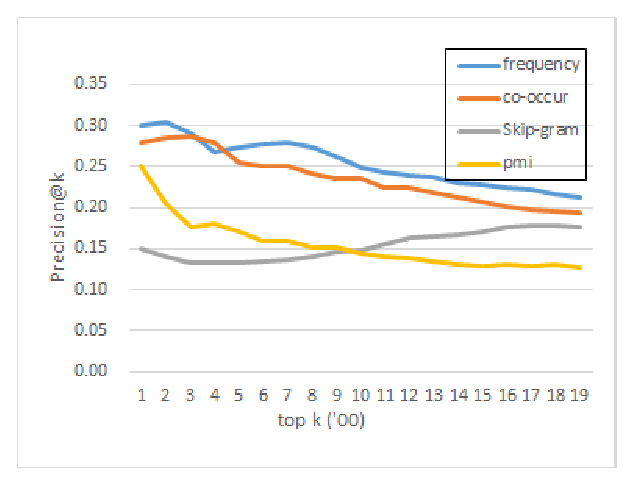
\includegraphics[width=0.32\textwidth]{img/precision}}\hfill
\subfloat[Recall curve]{\label{fig:recall_c}
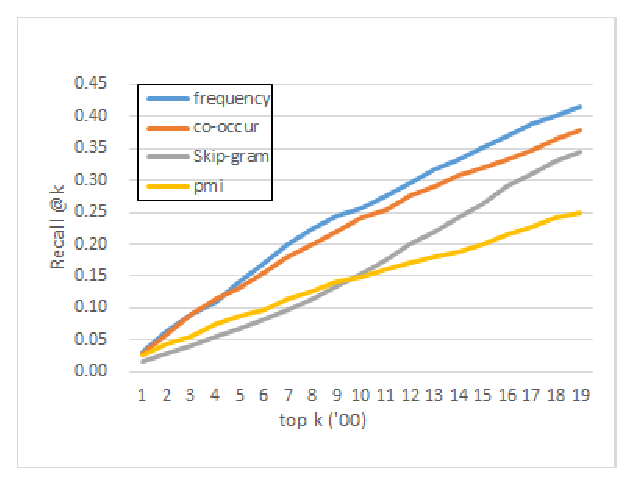
\includegraphics[width=0.32\textwidth]{img/recall}}\hfill
\subfloat[F1 curve]{\label{fig:f1_c}
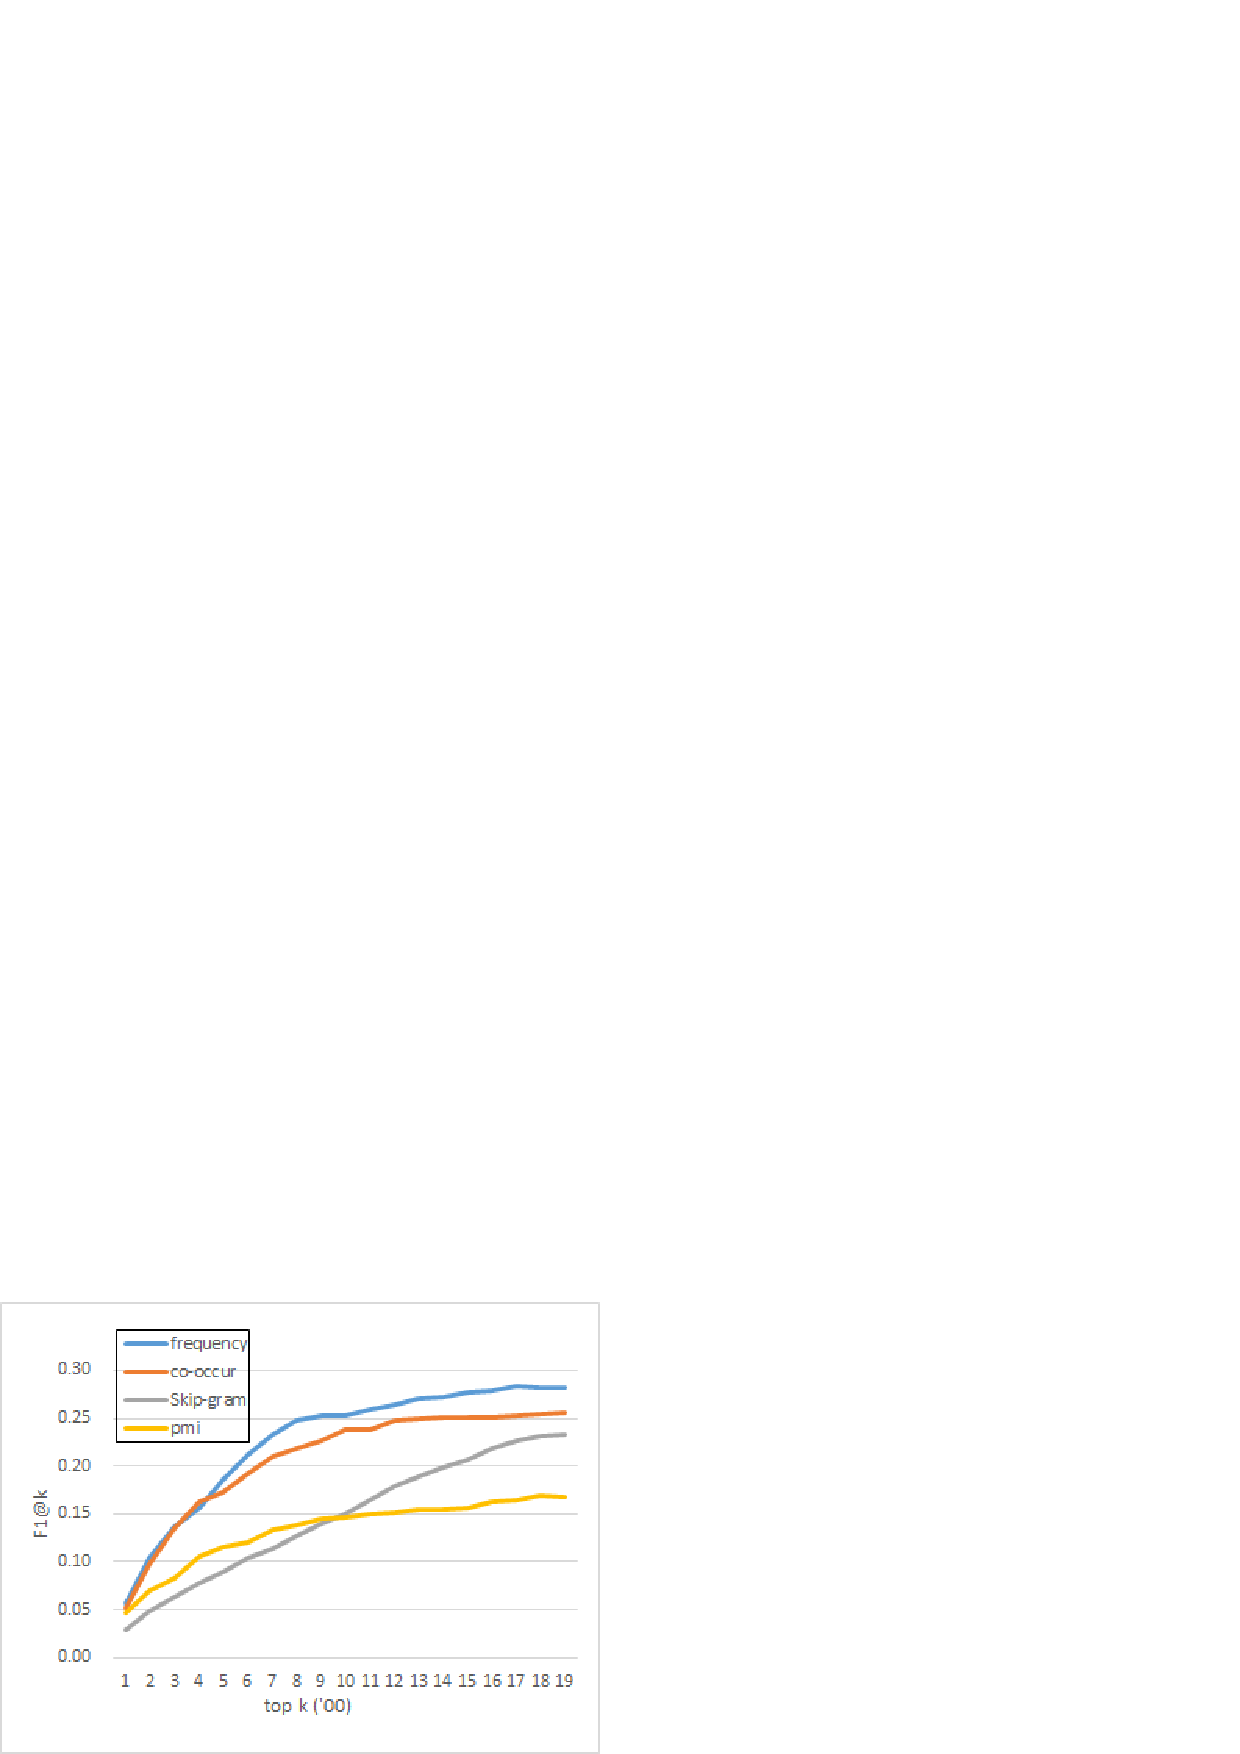
\includegraphics[width=0.32\textwidth]{img/F1}}
\caption{Precision, recall and F1-score for top $k$ words}
\label{fig:results}
\end{figure*}

\figref{fig:results} show the precision, recall and F1-score curves
with $k$ ranging from 1 to 1855,
for the three algorithms as well as the a random baseline.
Generally, the Skip-gram model has consistent advantage over the other
approaches by all three metrics. Among the co-occurrence based algorithms,
SVD algorithm outperforms the simple TF-IDF algorithm. However, both of these
are only better than the random algorithm for small $k$.

We argue that co-occurrence based algorithms underperform for three reasons.
First, cultural difference of a word may only be discovered by some very rare
words in the context. But TF-IDF favors more frequent and popular words and
gives those dimensions high weight. Consequently, this dilutes the weak
signals of cultural differences in many words.
For instance, consider the word
``football''. Assume that ``football'' co-occurs with ``Arsenal'' 10 times
in UK corpus and roughly 0 times in the US corpus. This is a significant
feature to show cultural difference, but is largely ignored due to the
small weight of ``Arsenal''.  Second, the co-occurrence
vector representation has very high dimension, and as a result, signals of
cultural difference on some of the dimensions maybe easily overwhelmed by
the similarity in other dimensions. Finally, according to the dictionaries,
many common words have many senses, and are more likely to have
cultural difference. However, the co-occurrence based methods tend to amplifify
the similarity for these common words and thus rank them lower.

%We think the reason is that some frequency-less words may be more important for supporting the meaning of aim word but this feature is easily ignored because of the overwhelmed number of more frequency words, which influences a great part of cosine similarity.  The other reason is that under co-occurrence based algorithm, the common words tend to have a bigger similarity. Even a common word has some cultural different meaning, if this meaning does not belong to the main meanings, the cosine similarity is still depended on the surrounding words of main meanings because of their predominant using rate. But another fact is that there are more cultural differences among common words defined in dictionary because both the public and the editors usually pay more attention on them.
%
%For TF-IDF co-occur algorithm and TF-IDF-SVD algorithm, which is an optimization for TF-IDF algorithm, we introduce TF-IDF of co-occur pairs to our problems. The applying of IF-IDF weakens the weight of common co-occur pairs, which leading to a more reasonable vector. The result shows this changing has a positive effect to some degree. However, to get a better result, the common words is still a limitation of IF-IDF's performance.
%

On the contrary, the Skip-gram model, though also making use of co-occurrences,
is good at capturing the fine signals in the context and amplify those signals
while ignoring the common and popular words in the surrounding. This is
possible due to the reduction of dimensionality by the neural network. We can
see the the precision of the Skip-gram model is high at low $k$ indicating
the quality of at the top of our list is very high.

\begin{table}
\small
\begin{tabular}{|c|c|c|c|c|c|}
\hline
Rank & Word & Hit? & Rank & Word & Hit?\\ \hline
\hline
1 & \bf{rook} & YES & 11 & moody & NO \\
\hline
2 & hardy & NO & 12 & {\bf mummy} & YES \\
\hline
3 & warlock & NO & 13 & finch & NO \\
\hline
4 & whilst & YES & 14 & chick & YES \\
\hline
5 & panther & YES & 15 & potter & YES \\
\hline
6 & harper & NO & 16 & fisher & YES \\
\hline
7 & fuller & NO & 17 & mar & NO \\
\hline
8 & \bf{united} & YES & 18 & \bf{wasp} & YES \\
\hline
9 & ulster & NO & 19 & quit & YES \\
\hline
10 & mole & NO & 20 & wan & NO \\
\hline
\end{tabular}
\caption{Top 20 culturally words by Skip-gram}
\label{tab:top20}
\end{table}

\tabref{tab:top20} lists the top 20 words returned by the Skip-gram model.
Under the ``Hits?'' column, ``Yes'' means this word is a true positive, while
``No'' means a false positive. The precision of these words is 0.5,
versus the actual percentage of positive
words in the input data, which is 0.279.

Also notice that some of the words
that are marked as false actually represent another kind of cultural
difference, in which a word means the same in the US and UK but is used in
different contexts or not used at all in one culture or another.
For example, ``ulster'' is a kind of northern Irish coat. In the US
corpus, we see it co-occurs with words like ``caption'', ``ship'' and
``boat'', which indicates this concept comes from outside of US.
While in the UK corpus, we see it co-occurs with words like ``sir'',
``man'', ``london'' and ``king'', which represents domestic affairs.
Such cultural differences are not reflected in our groundtruth.

\begin{table}
\small
\begin{tabular}{|c|c|c|}
\hline
Word & US meaning & UK meaning\\ \hline
\hline
{\bf rook} & European crow & firecracker \\
\hline
{\bf united} & Airlines & sports teams \\
\hline
{\bf mummy} & wrapped human body & mother \\
\hline
{\bf wasp} & White Anglo-Saxon Protestant & insect \\
\hline
\end{tabular}
\caption{Explanation of selected positive words}
\label{tab:explain}
\end{table}

\tabref{tab:explain} gives the explanation of four selected true positive
words returned by Skip-gram model according to the two dictionaries.
%The observation from the figures shows Wiktionary is more proper than Oxford Dictionary for our purposes. Because as an comprehensive resource, Oxford Dictionary contains a large number of informal meanings which never appear in publications.


